%----------------------------------------------------------------------------------
%	PACKAGES AND OTHER DOCUMENT CONFIGURATIONS
%----------------------------------------------------------------------------------
\documentclass[paper=a4, fontsize=12pt]{scrartcl} 	% A4 paper and 11pt font size

\usepackage[T1]{fontenc} 						% Use 8-bit encoding that has 256 glyphs
\usepackage{fourier} 							% Use the Adobe Utopia font for the document - comment this line to return to the LaTeX default
\usepackage[english]{babel} 						% English language/hyphenation
\usepackage{amsmath, amsfonts, amsthm, physics}
\usepackage{graphicx}
\usepackage{indentfirst}
\setlength\parindent{20pt}
\usepackage{sectsty} 							% Allows customizing section commands
\allsectionsfont{\normalfont\scshape} 		% Make all sections centered, the default font and small caps

\usepackage{fancyhdr} 							% Custom headers and footers
\pagestyle{fancyplain} 							% Makes all pages in the document conform to the custom headers and footers
\fancyhead[L]{Physics 127B, Mazin}
\fancyhead[R]{Monte Mishkin}
\fancyfoot[C]{}
\fancyfoot[R]{\thepage} 							% Page numbering for right footer
\renewcommand{\headrulewidth}{0pt} 				% Remove header underlines
\renewcommand{\footrulewidth}{0pt} 				% Remove footer underlines
\setlength{\headheight}{13.6pt} 					% Customize the height of the header

\newcommand{\horrule}[1]{\rule{\linewidth}{#1}} 		% Create horizontal rule command with 1 argument of height

\newcommand{\mm}[1]{\fontfamily{\ttdefault}\selectfont#1\fontfamily{\rmdefault}\selectfont}



%----------------------------------------------------------------------------------
%	TITLE SECTION
%----------------------------------------------------------------------------------
\begin{document}
\begin{center}
	\huge Final Project\\[0.4cm]
	\small March 13, 2015
	\horrule{0.5pt} \\[0.4cm]
\end{center}

%----------------------------------------------------------------------------------
%        DOCUMENT
%----------------------------------------------------------------------------------

\begin{abstract}
	I built some external circuitry to send sound, light, and orientation data to my Arduino.  The Arduino does some initial processing of this data before sending it to my computer over a serial port.  I then designed a rudimentary program structure in Processing which could be used to render visuals based on the data received by the Arduino.  Finally, I wrote two separate implementations of this design, one in 2D, and one in 3D.
\end{abstract}


%----------------------------------------------------------------------------------


\section{The Circuitry}
	Figure \ref{mic} shows the circuitry responsible for sending the sound data to the Arduino.  This is not a course on analog electronics so I will not go into detail (the circuit is adapted from page 204 in the lab manual, where there is indeed an explanation).  Essentially, the microphone signal is boosted by a single-supply op amp.  This signal has some serious fuzz, so it is sent through a low-pass filter.  Finally, a switch controls whether the Arduino pin $A2$ reads the microphone signal or just ground.  This allows the user to disable the sound-based visualizations if desired.
	
	Figure \ref{buttons} shows the circuitry responsible for monitoring the left and right buttons.  It is pretty self-explanatory.  The readings are normally LOW unless the buttons are pressed.
	
	Figure \ref{light} shows the circuitry responsible for sending the light data to the Arduino.  It too is rather self-explanatory.  The photo-resistor changes its resistance based on the amount of light it receives.  Thus placing it in a simple voltage divider causes the output to vary between ground and $V_{cc}$ based on the amount of light received.  As it is wired here, more light means higher voltage.  A switch controls whether the Arduino pin $A0$ reads the light signal or just $V_{cc}$.  This allows the user to disable the light-based visualizations if desired.
	
	Figure \ref{switch} shows a simple switch circuit.  This is entirely self-explanatory.  Its purpose is open to interpretation from the hardware point of view.  In my 3D implementation its purpose is to allow the user to decide whether or not the motion data should move the camera through the 3D scene.
	
	Figure \ref{mpu} shows a the wiring for the MPU (motion processing unit).  Other than the obvious power connections, the MPU's $SDA$ and $SCL$ pins are connected to Arduino pins $A4$ and $A5$.  These Arduino pins correspond to $SDA$ (serial data) and $SCL$ (serial clock) for using I2C devices, in my Arduino board's documentation.  The MPU's $INT$ (interrupt) pin is linked to the Arduino's $D2$ pin (which is the external interrupt pin for my Arduino board).


%----------------------------------------------------------------------------------


\section{The Arduino Code}
	I tried my best to make the code self documented, so here I will just give the basic idea behind the program.  The Arduino code for both the 2D and 3D implementations is extremely similar (maybe 3 lines different).  Thus I will go over the 2D code and then tell you what is different about the 3D code.  
	
	In the "pepper/arduino/v3/" directory there are three files.  In "v3.ino" I have placed all of the code which "builds the desired programming environment".  This includes things like library imports, preprocessor directives, global variable declarations, and helper functions.  
	
	Next is the "Setup.ino" file where I define the setup routine.  I sincerely hope that the code here is sufficiently self-documented and self-explanatory.  
	
	Finally, we have the file "Loop.ino" where I define the routine that is to be repeated by the micro-controller.  The design here (and in "Setup.ino") is an extension / reformulation of some of the examples found on the website for the "I2Cdev" library I used.  Basically, we have a lot of clutter going on to make sure that the MPU is working correctly.  Ignoring this, however, the key idea is that the loop needs to taylor itself towards properly receiving and processing the MPU's data.  The other sensors are all secondary to this, and must only have their readings updated while the MPU is doing its own processing (and is hence not triggering an interrupt to send data, or having any other sort of problem).  Of course, this design is not \emph{vital}, it's just that it produces better results since the most finicky of the sensors is the motion sensor.  This however has the very unfortunate side effect that the sound readings are much slower than if there was no interruption scheme in effect.
	
	Anyways, the only difference between the 2D and 3D Arduino code is that the 3D code makes one additional reading for the simple switch.  The 2D visualizations do not make use of this switch and hence do not require it in the Arduino code.

%----------------------------------------------------------------------------------


\section{The Processing Code}
	Again, I tried my best to make the code self documented, so here I will just give the basic idea behind the program.  As mentioned before, I made two separate implementations of a single common design.  First I will talk about the design and then the two implementations.  Just so that you know for later, I titled the 2D implementation "Pepper" and the 3D implementation "Starfire".
	
\subsection{The Common Design}
	Just to have something concrete to look at, let's take a look into the "starfire/processing/v6/" directory.  In "Main.pde" I have placed the four most important functions: \mm{setup}, \mm{draw}, \mm{serialEvent}, and \mm{update\_globals}. 
	 
	The \mm{setup} function is called once at the beginning of the program.  It does things like size the display and prepare the serial port for communication.  It also is responsible for preparing all of the rest of the data structures to be used later in the program.
	
	The \mm{serialEvent} function is called every time a full line of serial data is received (every newline character).  It is responsible for doing preliminary processing of this serial data.  For instance, if the data is in the expected (comma-separated value) format, the \mm{serialEvent} function parses the data and stores it into various global variables.  Another key feature of the \mm{serialEvent} function is that it updates the global \mm{LAST\_SERIAL\_TIME} which stores the timestamp of the most recent serial event.  Note that in addition to this, the \mm{serialEvent} function can set two flags.  If it has received properly formatted serial data, it sets \mm{SERIAL\_READY} to true.  Furthermore, if this (properly formatted) serial data is the first such data to be received, it sets \mm{SERIAL\_BEGUN} to true.  More on these flags later.
	
	The \mm{draw} function is then called repeatedly.  It is responsible for rendering and iterating the content, whatever that may be.  The \mm{draw} function also has two other key responsibilities.  First of all, it checks to make sure that the last serial event did not occur too long (one second) ago.  If it did, we try to reconnect.  Secondly, \mm{draw} checks to see if there is serial data ready for post processing (if \mm{SERIAL\_READY} is true).  If it is, it updates any global variables which store some value that requires a calculation based on the latest serial data.  The justification for this taking place outside of \mm{serialEvent} is that, these calculations might take up time and slow down the reception of the serial data.  Since they only need to happen each draw frame (rather than each serial event) it is best to put them there and leave the serial event rate as un-touched as possible.  As a little side, I added a simple loading screen.  This is what the \mm{SERIAL\_BEGUN} flag is for.  If the first (properly formatted) serial data has not yet been received, the loading screen is displayed, which logs information about the current hardware and software status.
	
	That's basically it.  The only other main thing that is common to both implementations is the \mm{FloatBuffer} class (found in "FloatBuffer.ino").  I wrote this class to log the sound data over time.  Then I realized that it should really be used for any analog (or digital, really) data that is to be watched over time.  Basically, it just provides a convenient way of storing the most recent few readings for the relevant data.  That's all.


\subsection{The 2D Implementation - Pepper}
	Pepper is a stupid 2D game with no objective.  You are a finch, and there are monsters.  That's about it.  The MPU orientation determines which direction you move in.  The right button allows you to hop, the left to fly.  The light determines the backdrop.  The sound draws the grass on the ground.  That's about all.  I'm not sure how in-depth you want me to go on this so I'll just stop here, but if you want more of an explanation I would be happy to provide it (the same goes for the rest of my project in its entirety).


\subsection{The 3D Implementation - Starfire}
	Starfire is kind of a game.  But only kind of.  Again there is no objective.  There is a colorful platform that changes color in time.  I wrote a DE (similar to the heat equation) which determines how the color changes in time.  The orientation of the MPU determines several of the "constants" in this DE, so that the way the colors change is determined by the motion of the controller.  The motion of the controller also moves the character through the 3D scene (unless you have flicked the switch to disable this).  With no buttons pressed, you can move forward, backward, left and right.  With the right button pressed you can move up, down, left, and right.  With the left button pressed you can look around but not move.  The sound data is displayed in a ring surrounding the colorful platform.  The light data determines the 3D lighting effects applied to the scene.  There are also two simulations taking place which do \emph{not} depend on any of the data being received.  I included these (everything that is colored white) to demonstrate how one should differentiate in the programing between events which do and do not depend on the serial data.  Also, when you press both buttons, the simulation is reset.  


%----------------------------------------------------------------------------------
	

\begin{figure}
	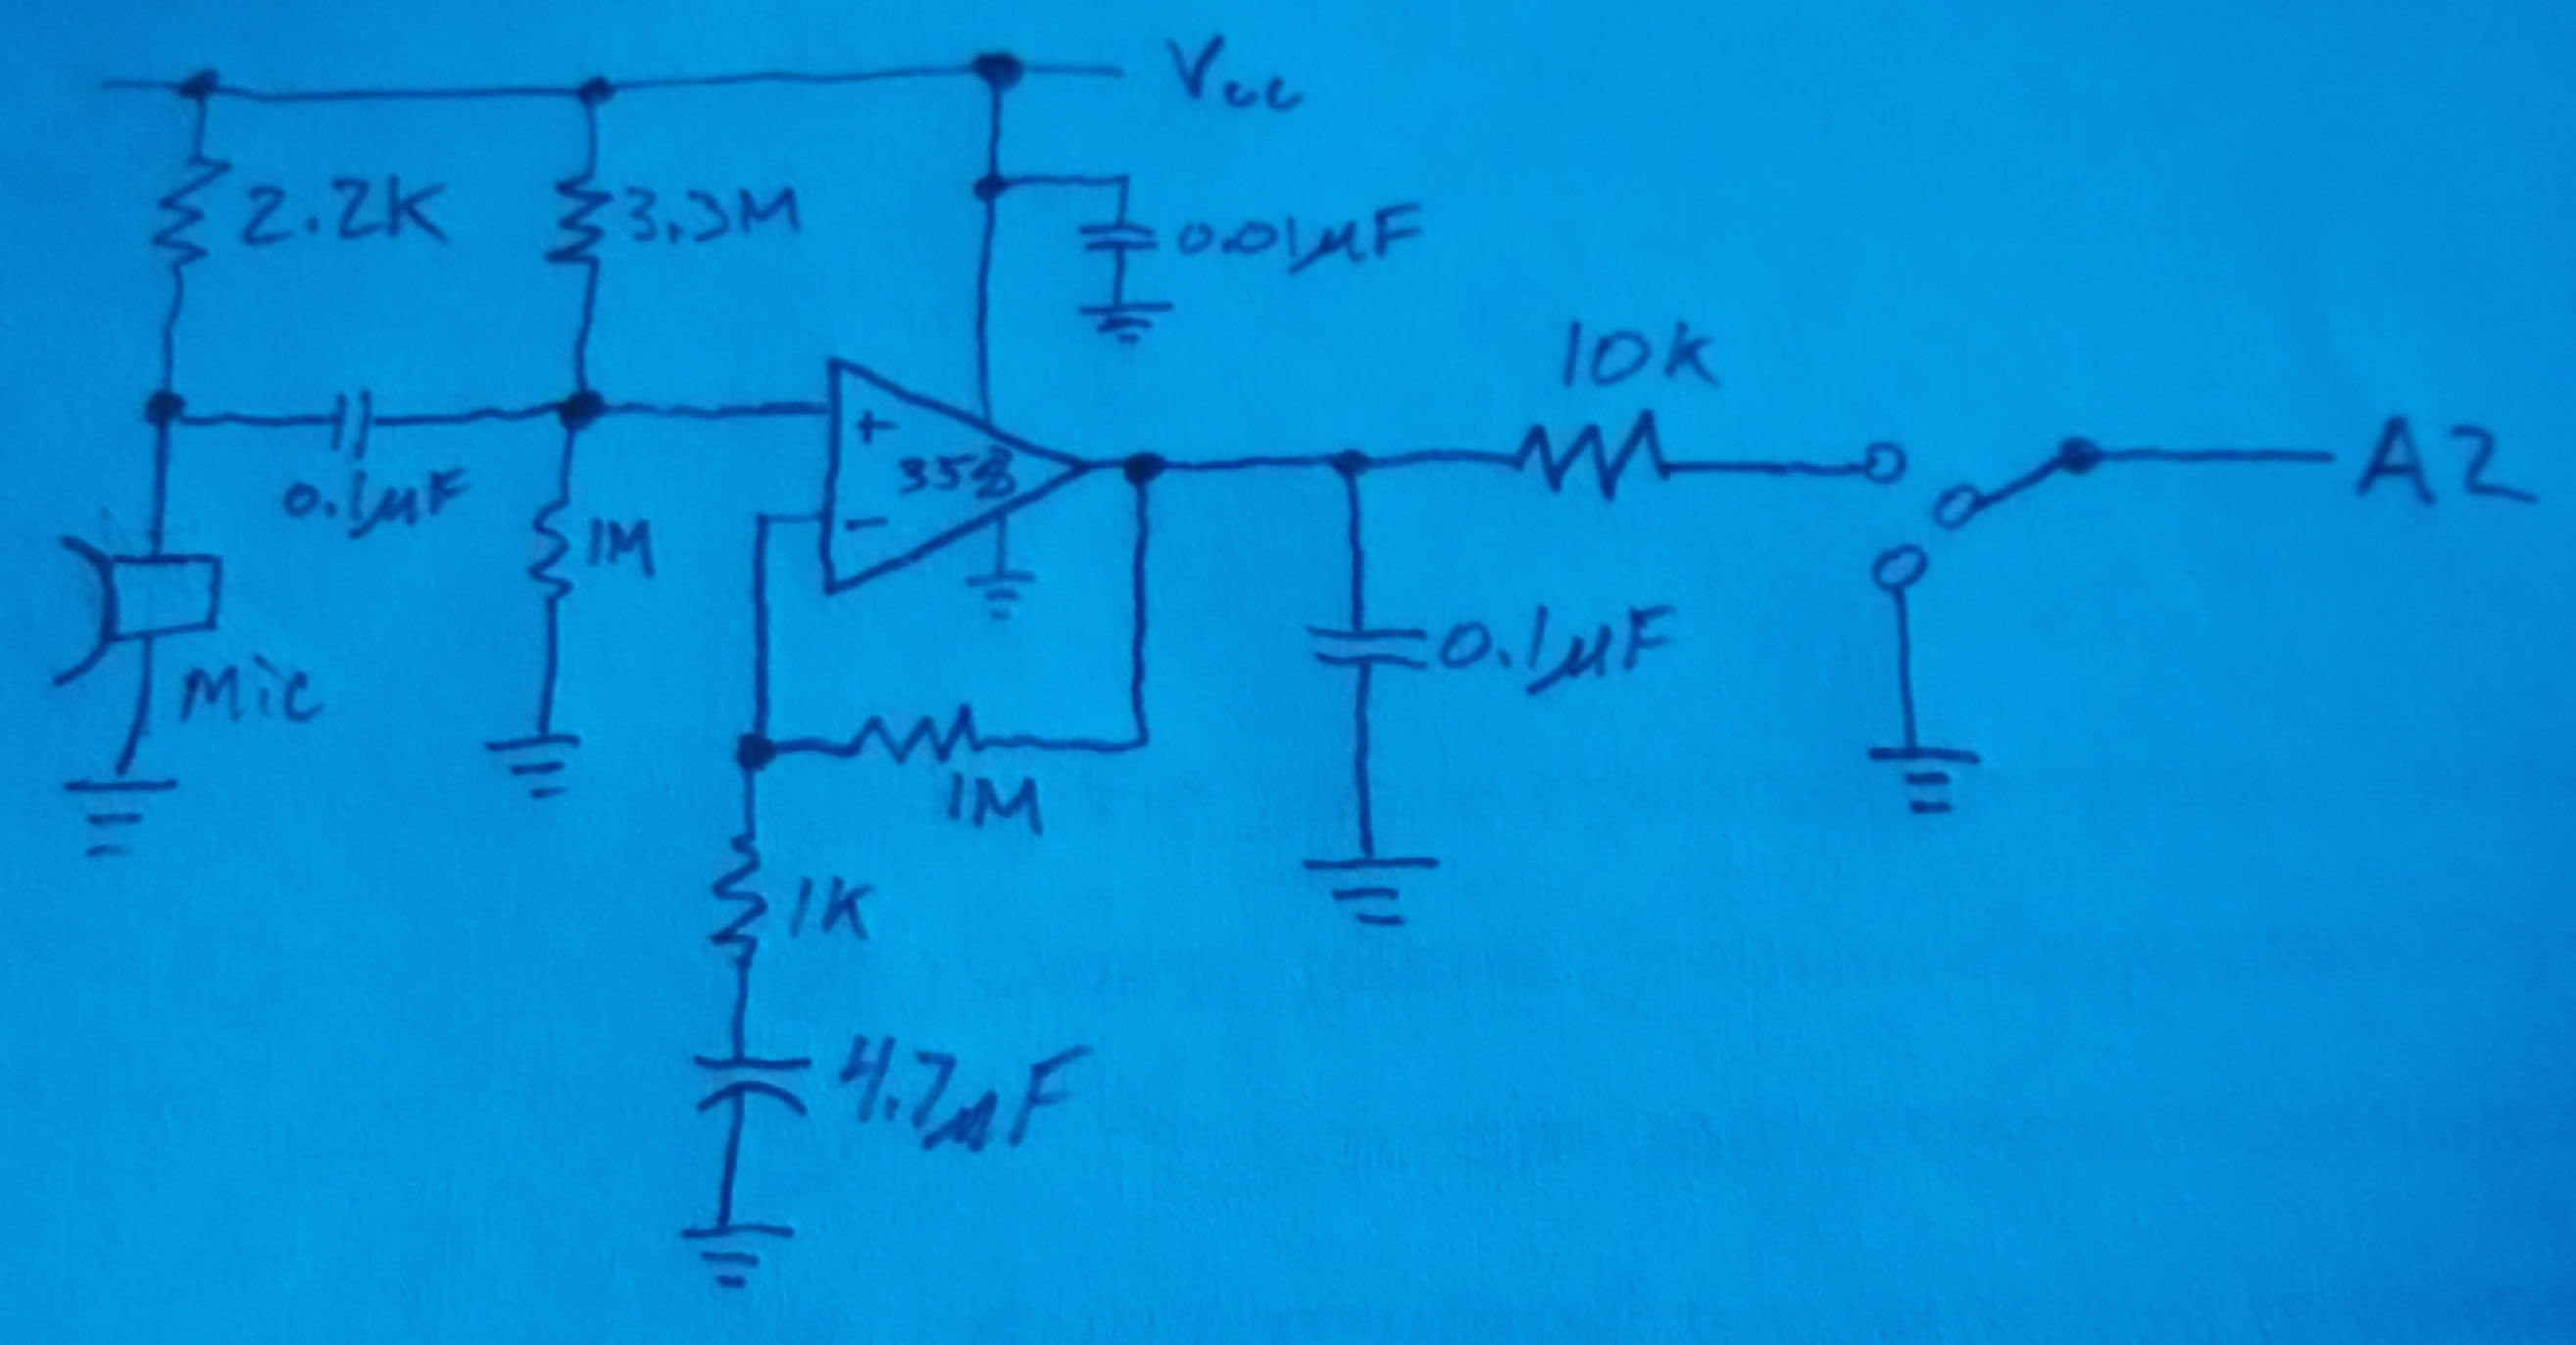
\includegraphics[scale=0.14]{mic.jpg}
	\caption{\label{mic} Circuit diagram of microphone, amplifier, and filter.  Sent to Arduino pin $A2$.}
\end{figure}

\begin{figure}
	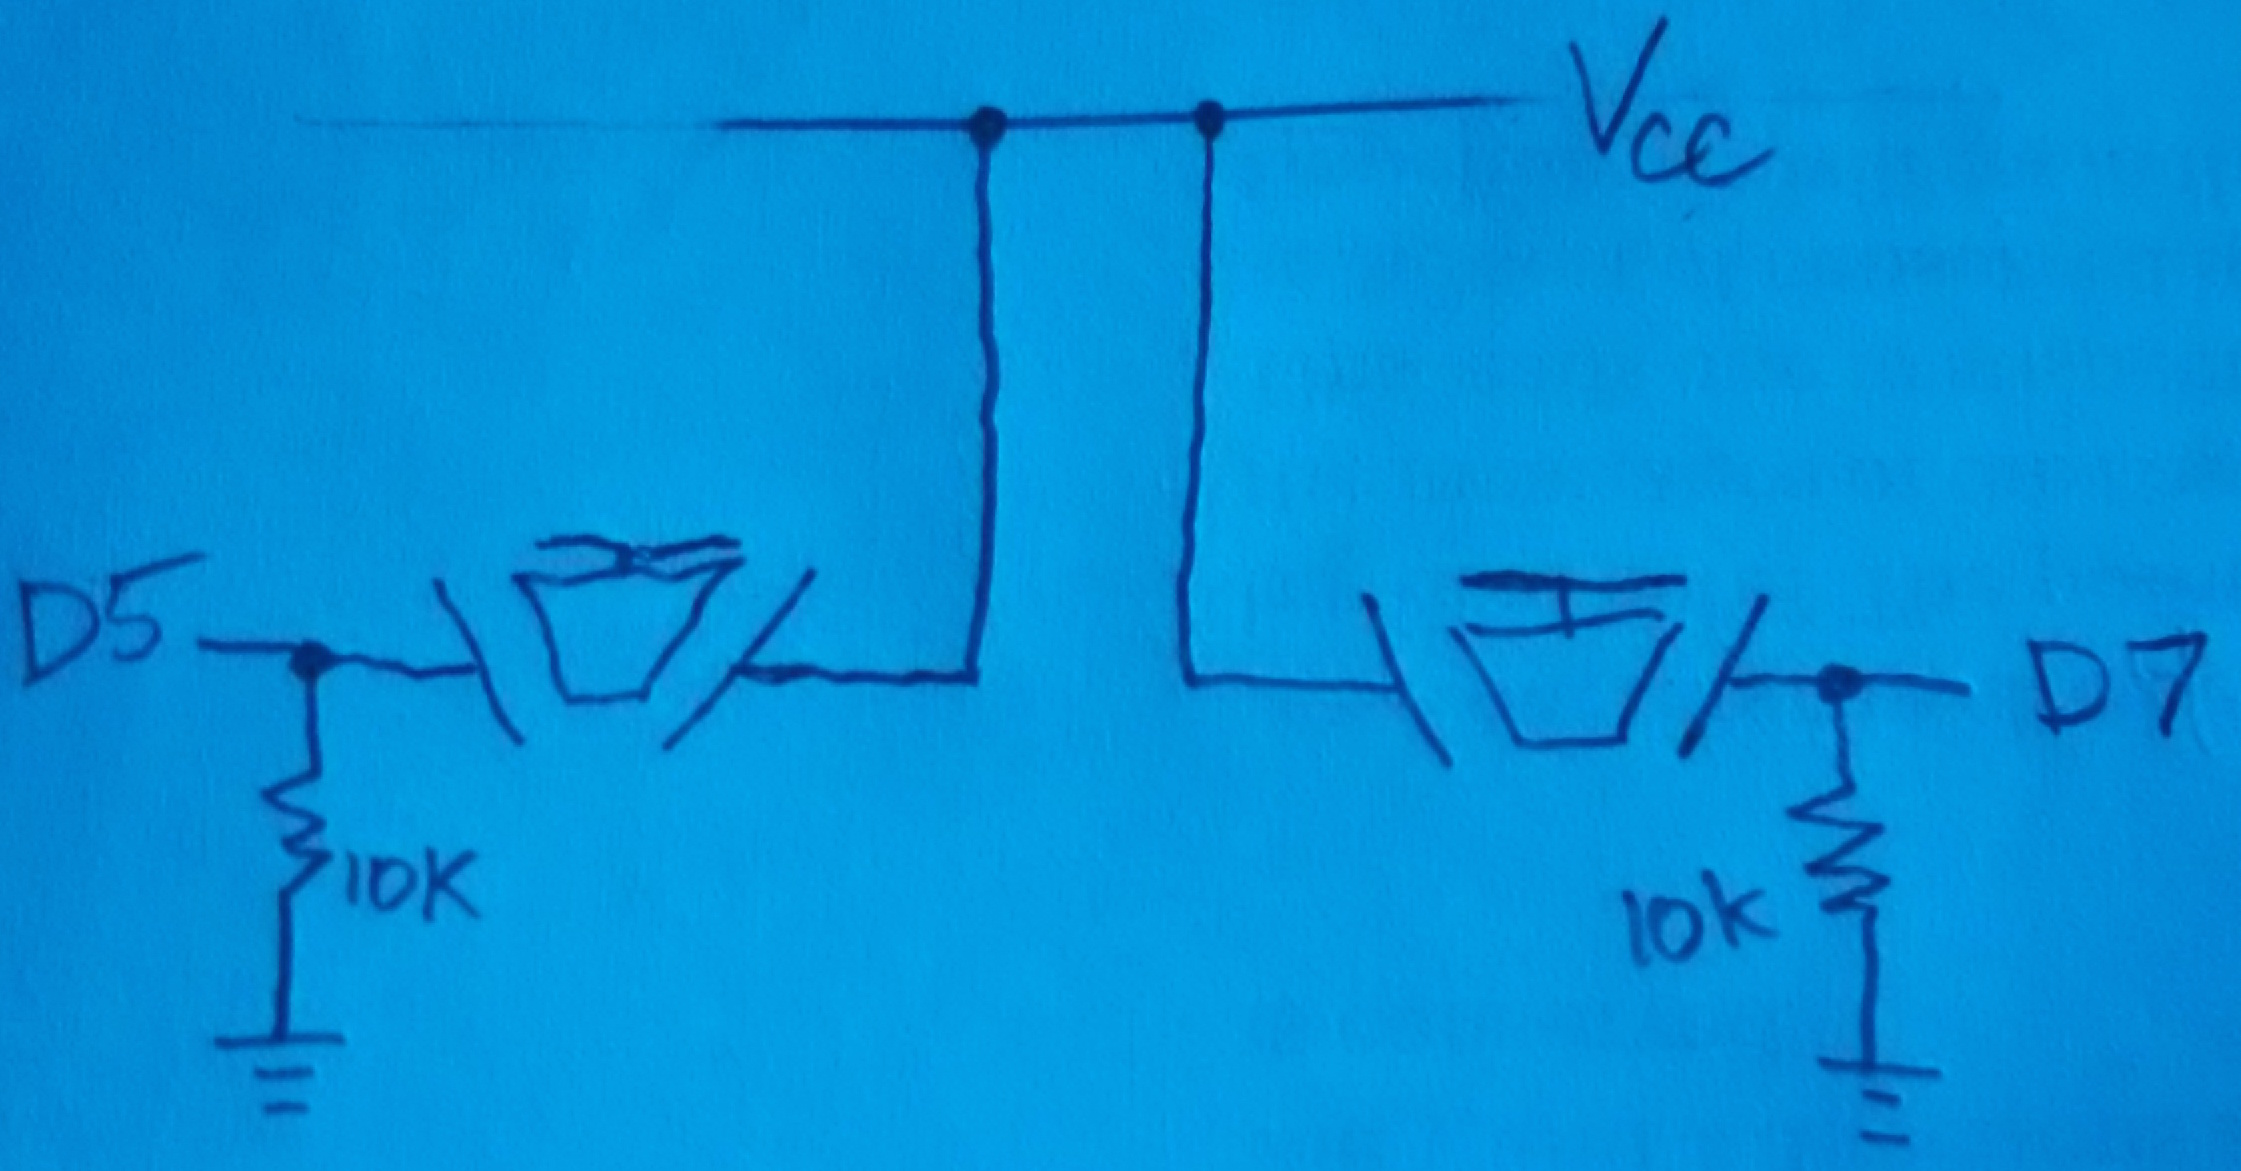
\includegraphics[scale=0.16]{buttons.jpg}
	\caption{\label{buttons} Circuit diagram of left and right buttons.  Sent to Arduino pins $D5$ and $D7$.}
\end{figure}

\begin{figure}
	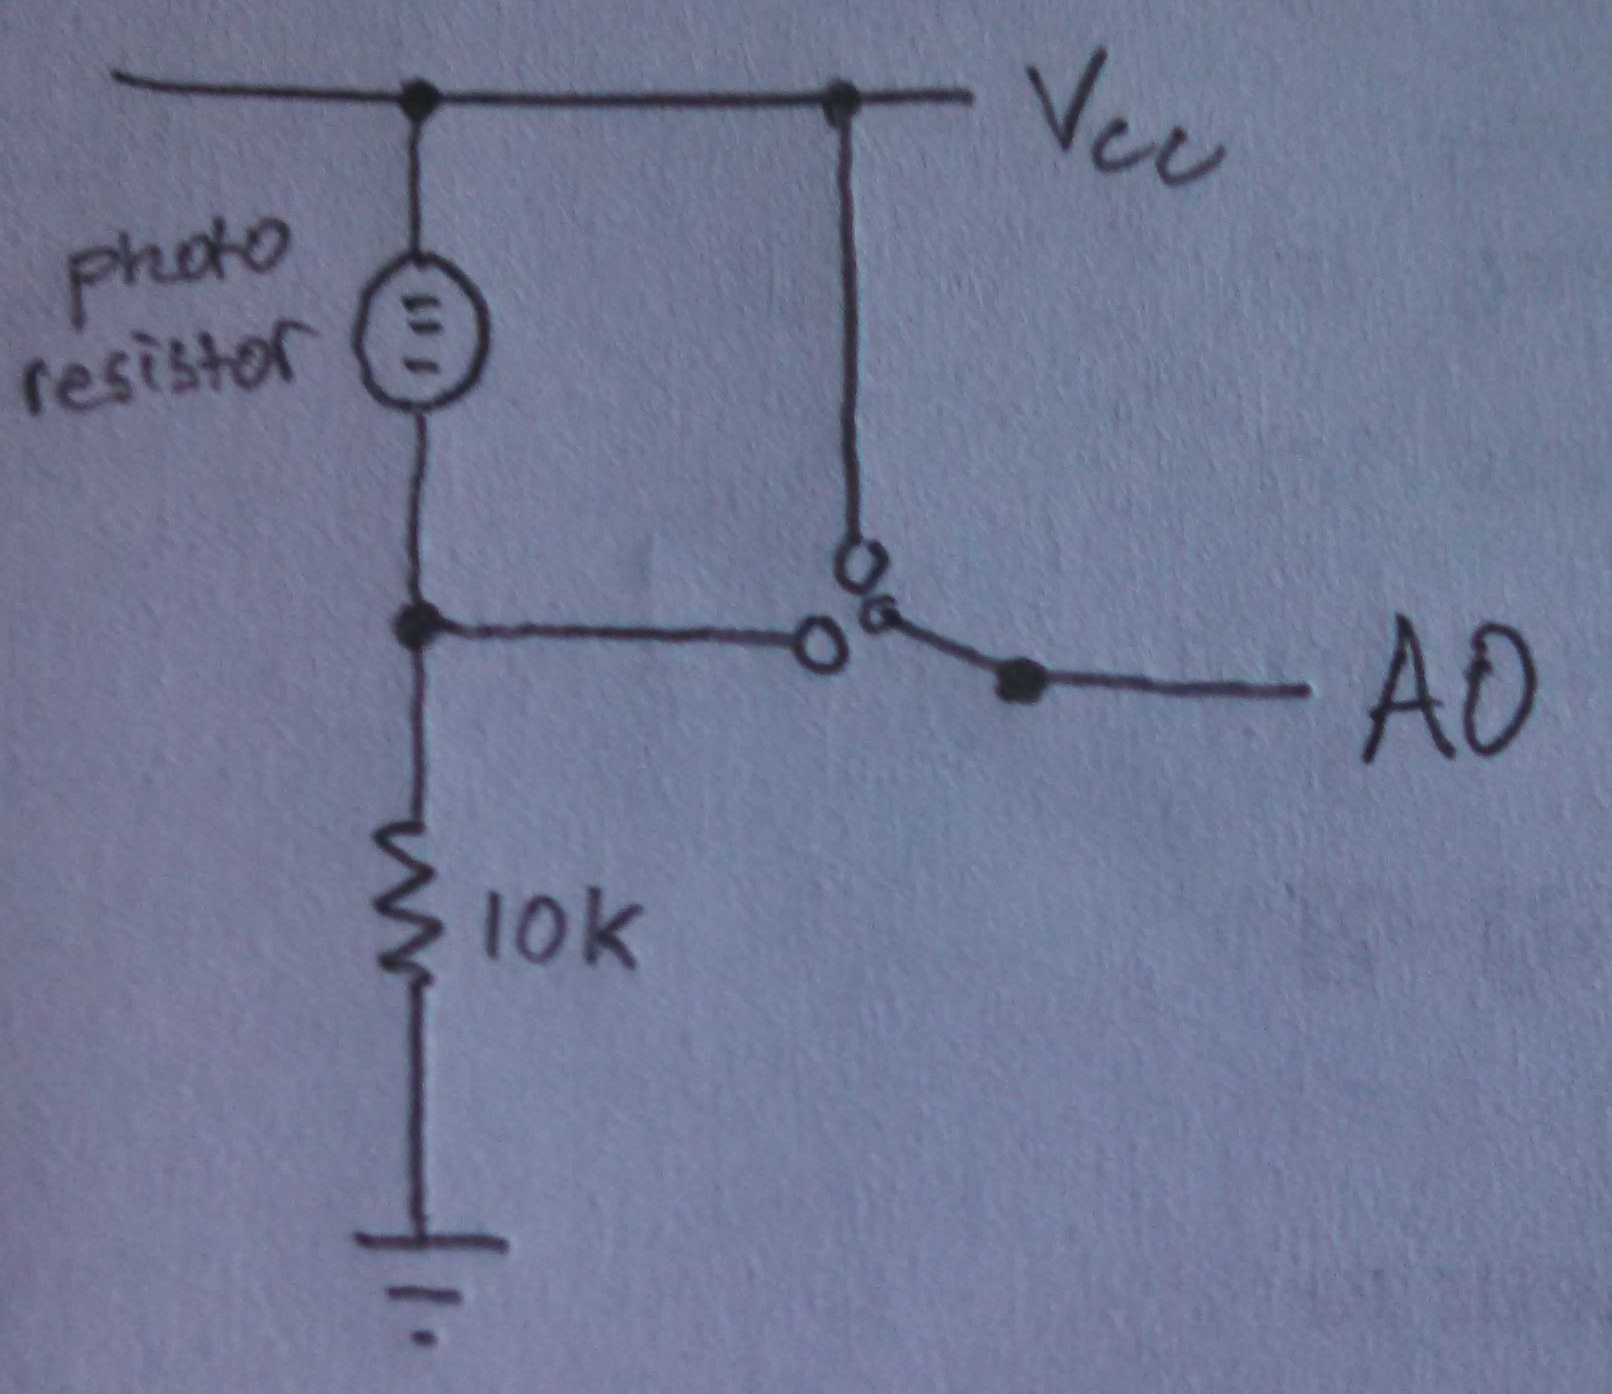
\includegraphics[scale=0.16]{light.jpg}
	\caption{\label{light} Circuit diagram of light sensor.  Sent to Arduino pin $A0$.}
\end{figure}

\begin{figure}
	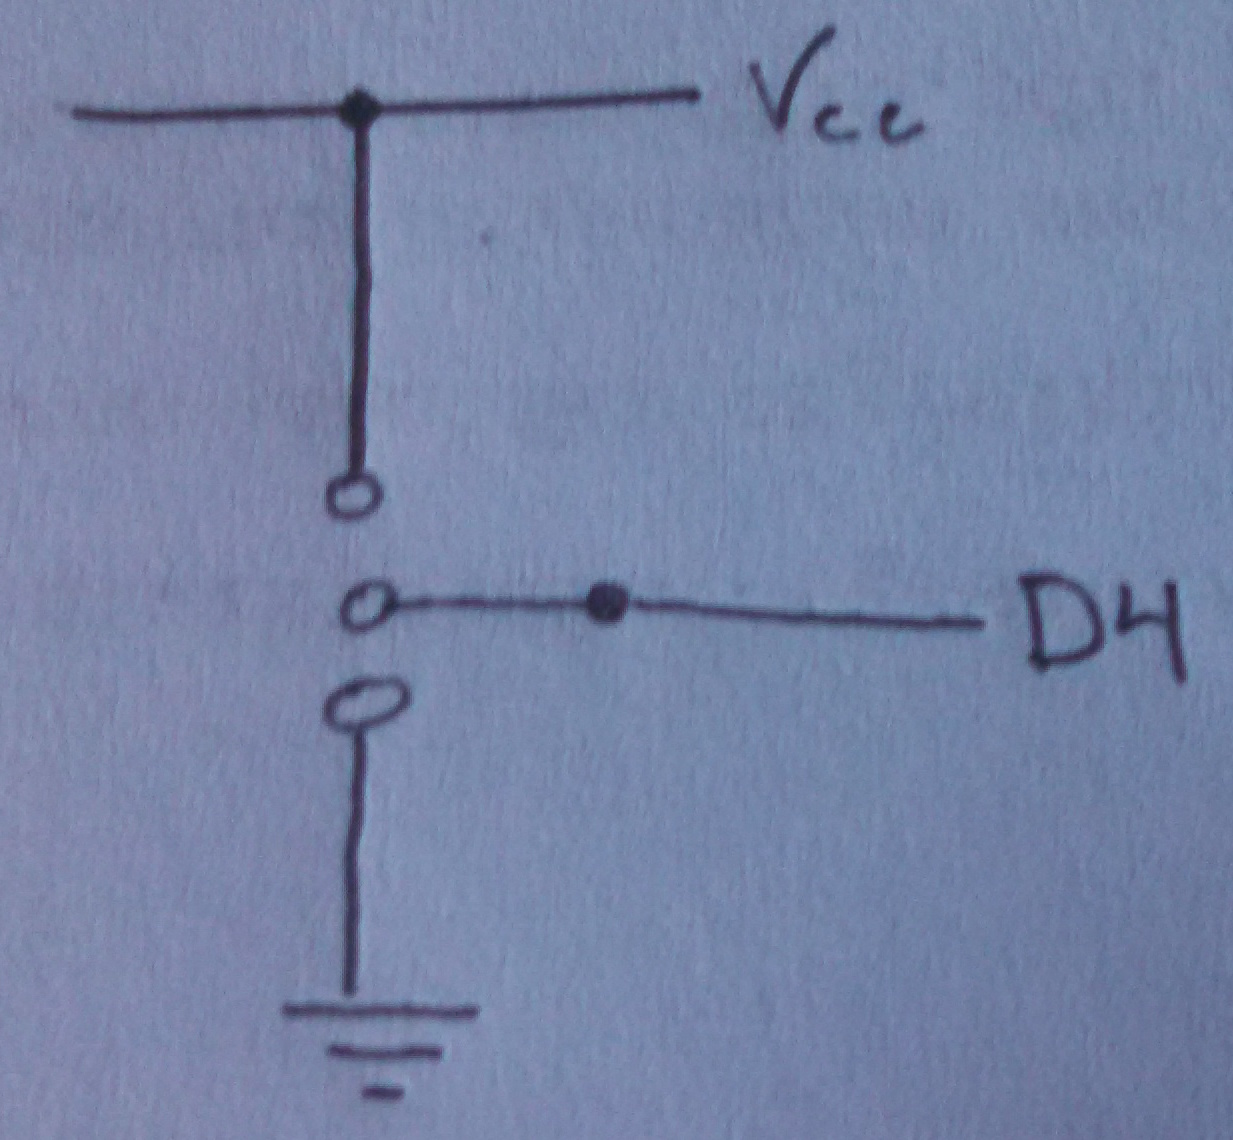
\includegraphics[scale=0.16]{switch.jpg}
	\caption{\label{switch} Circuit diagram of switch.  Sent to Arduino pin $D4$.}
\end{figure}

\begin{figure}
	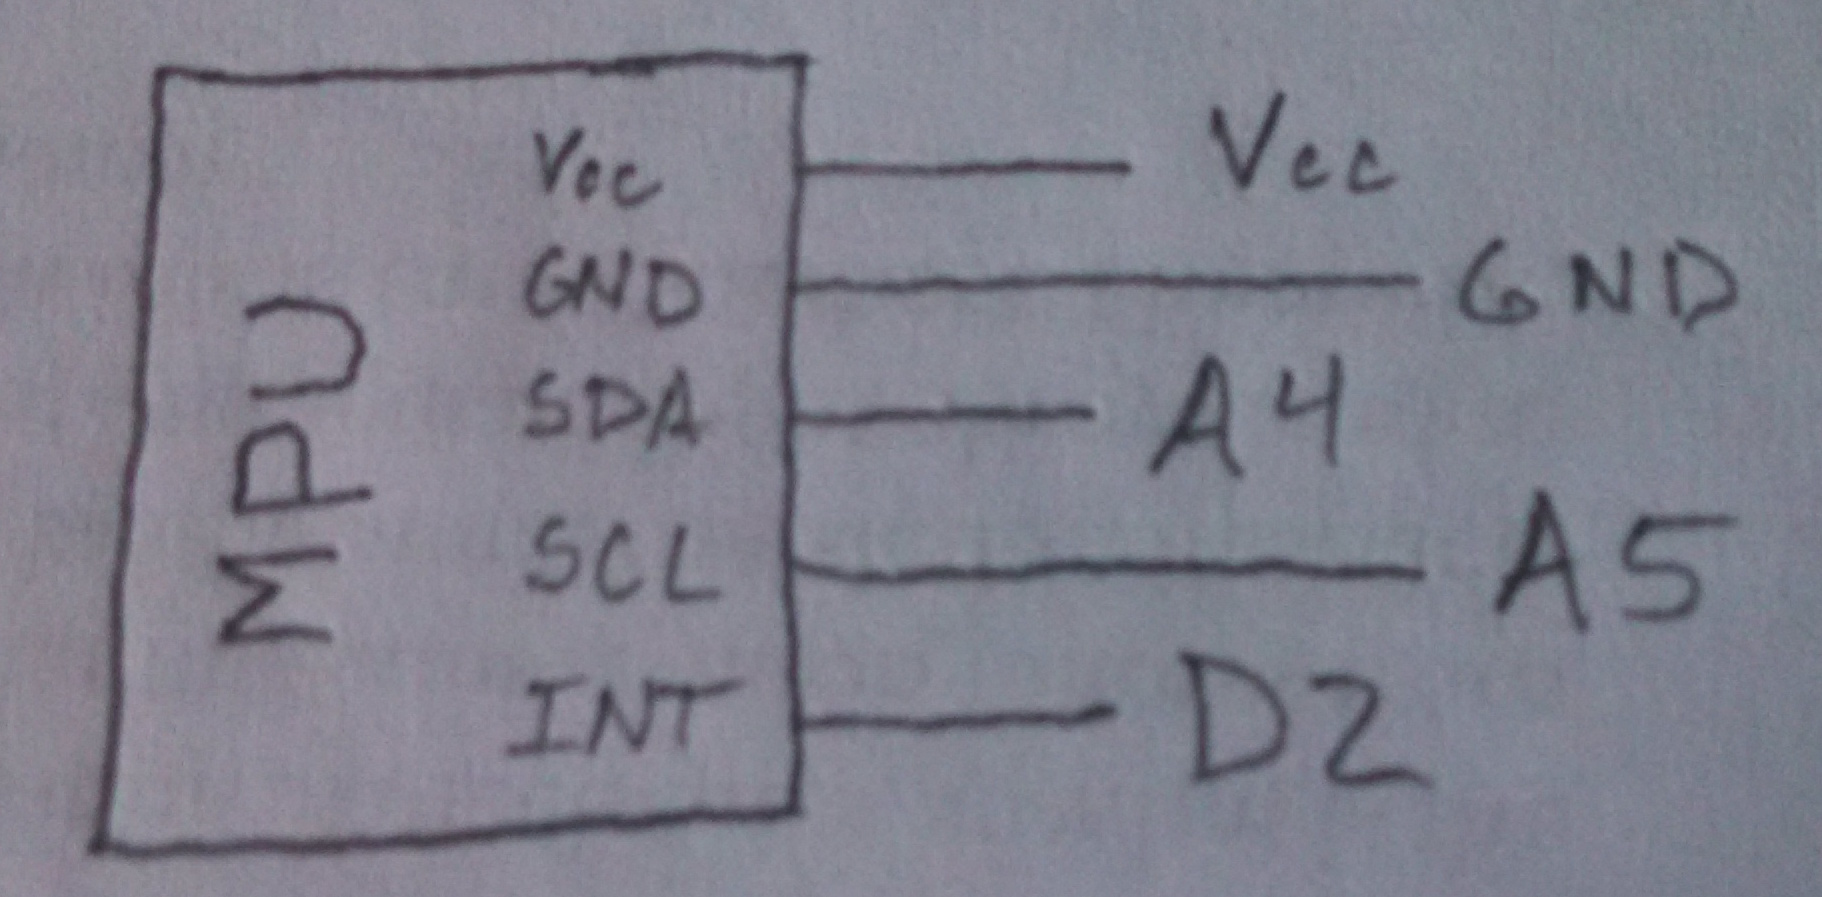
\includegraphics[scale=0.16]{mpu.jpg}
	\caption{\label{mpu} Circuit diagram of MPU.}
\end{figure}

\begin{figure}
	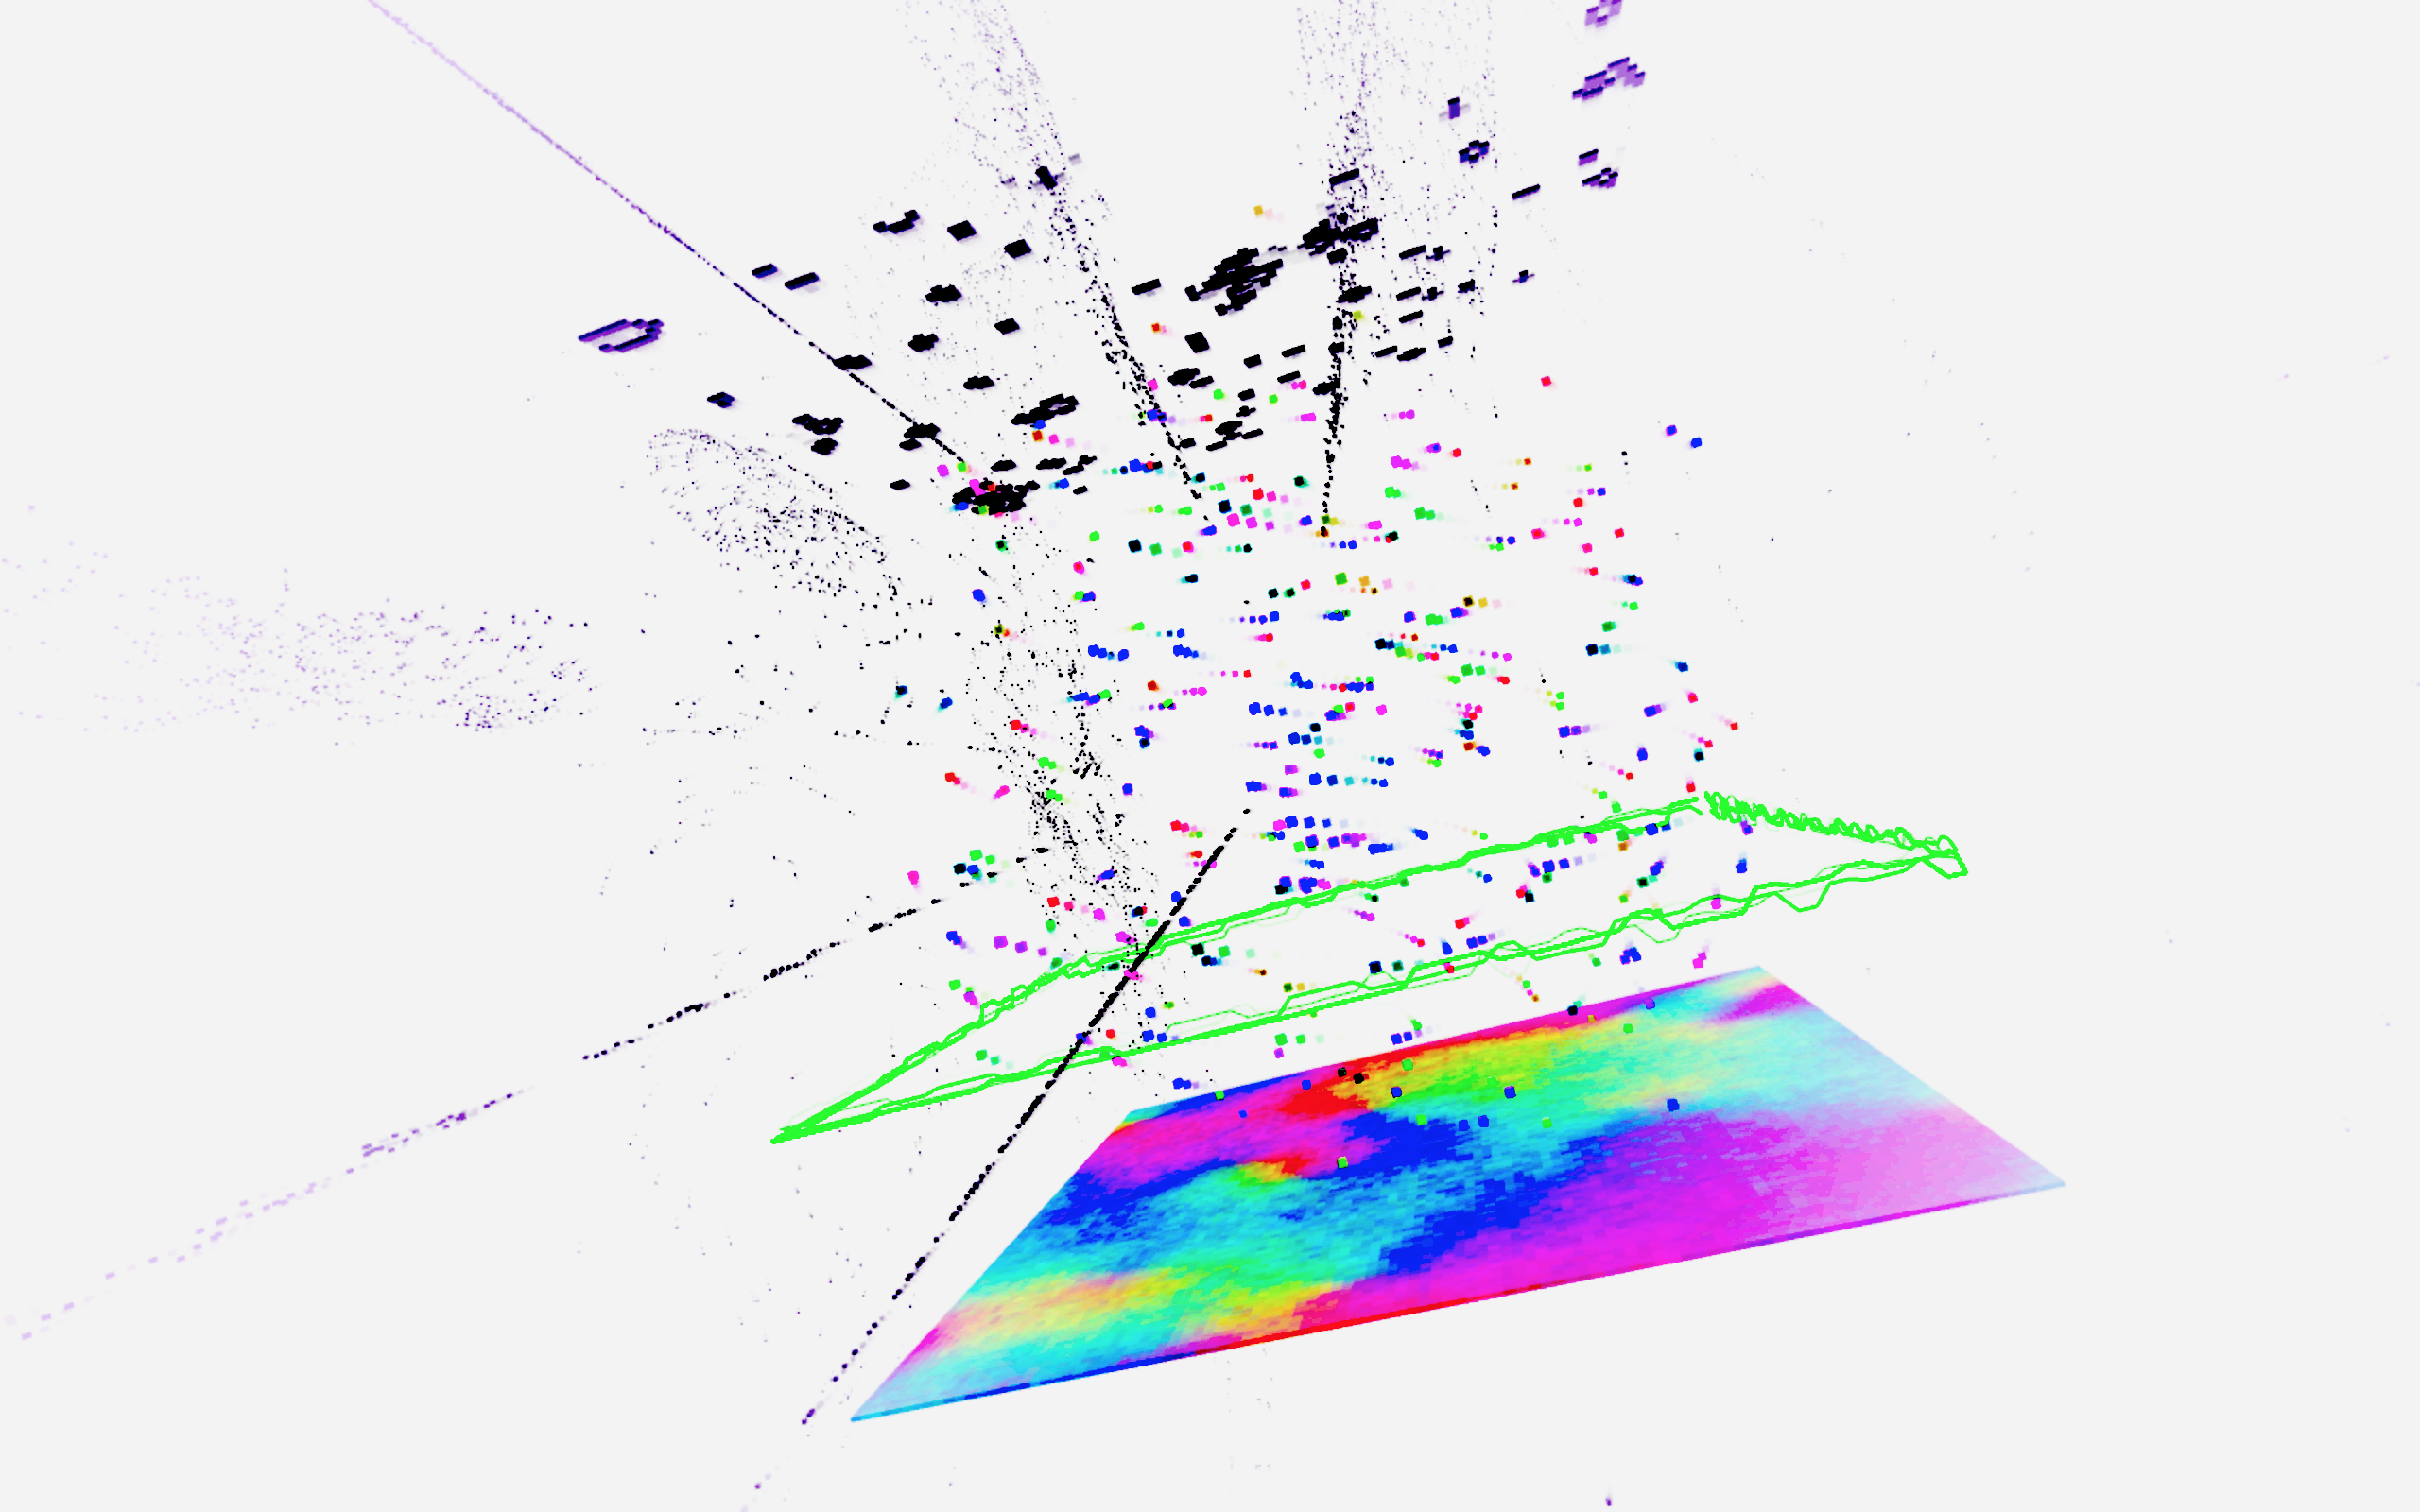
\includegraphics[scale=0.3]{starfire.png}
	\caption{\label{starfire} Screenshot from "Starfire".}
\end{figure}

\begin{figure}
	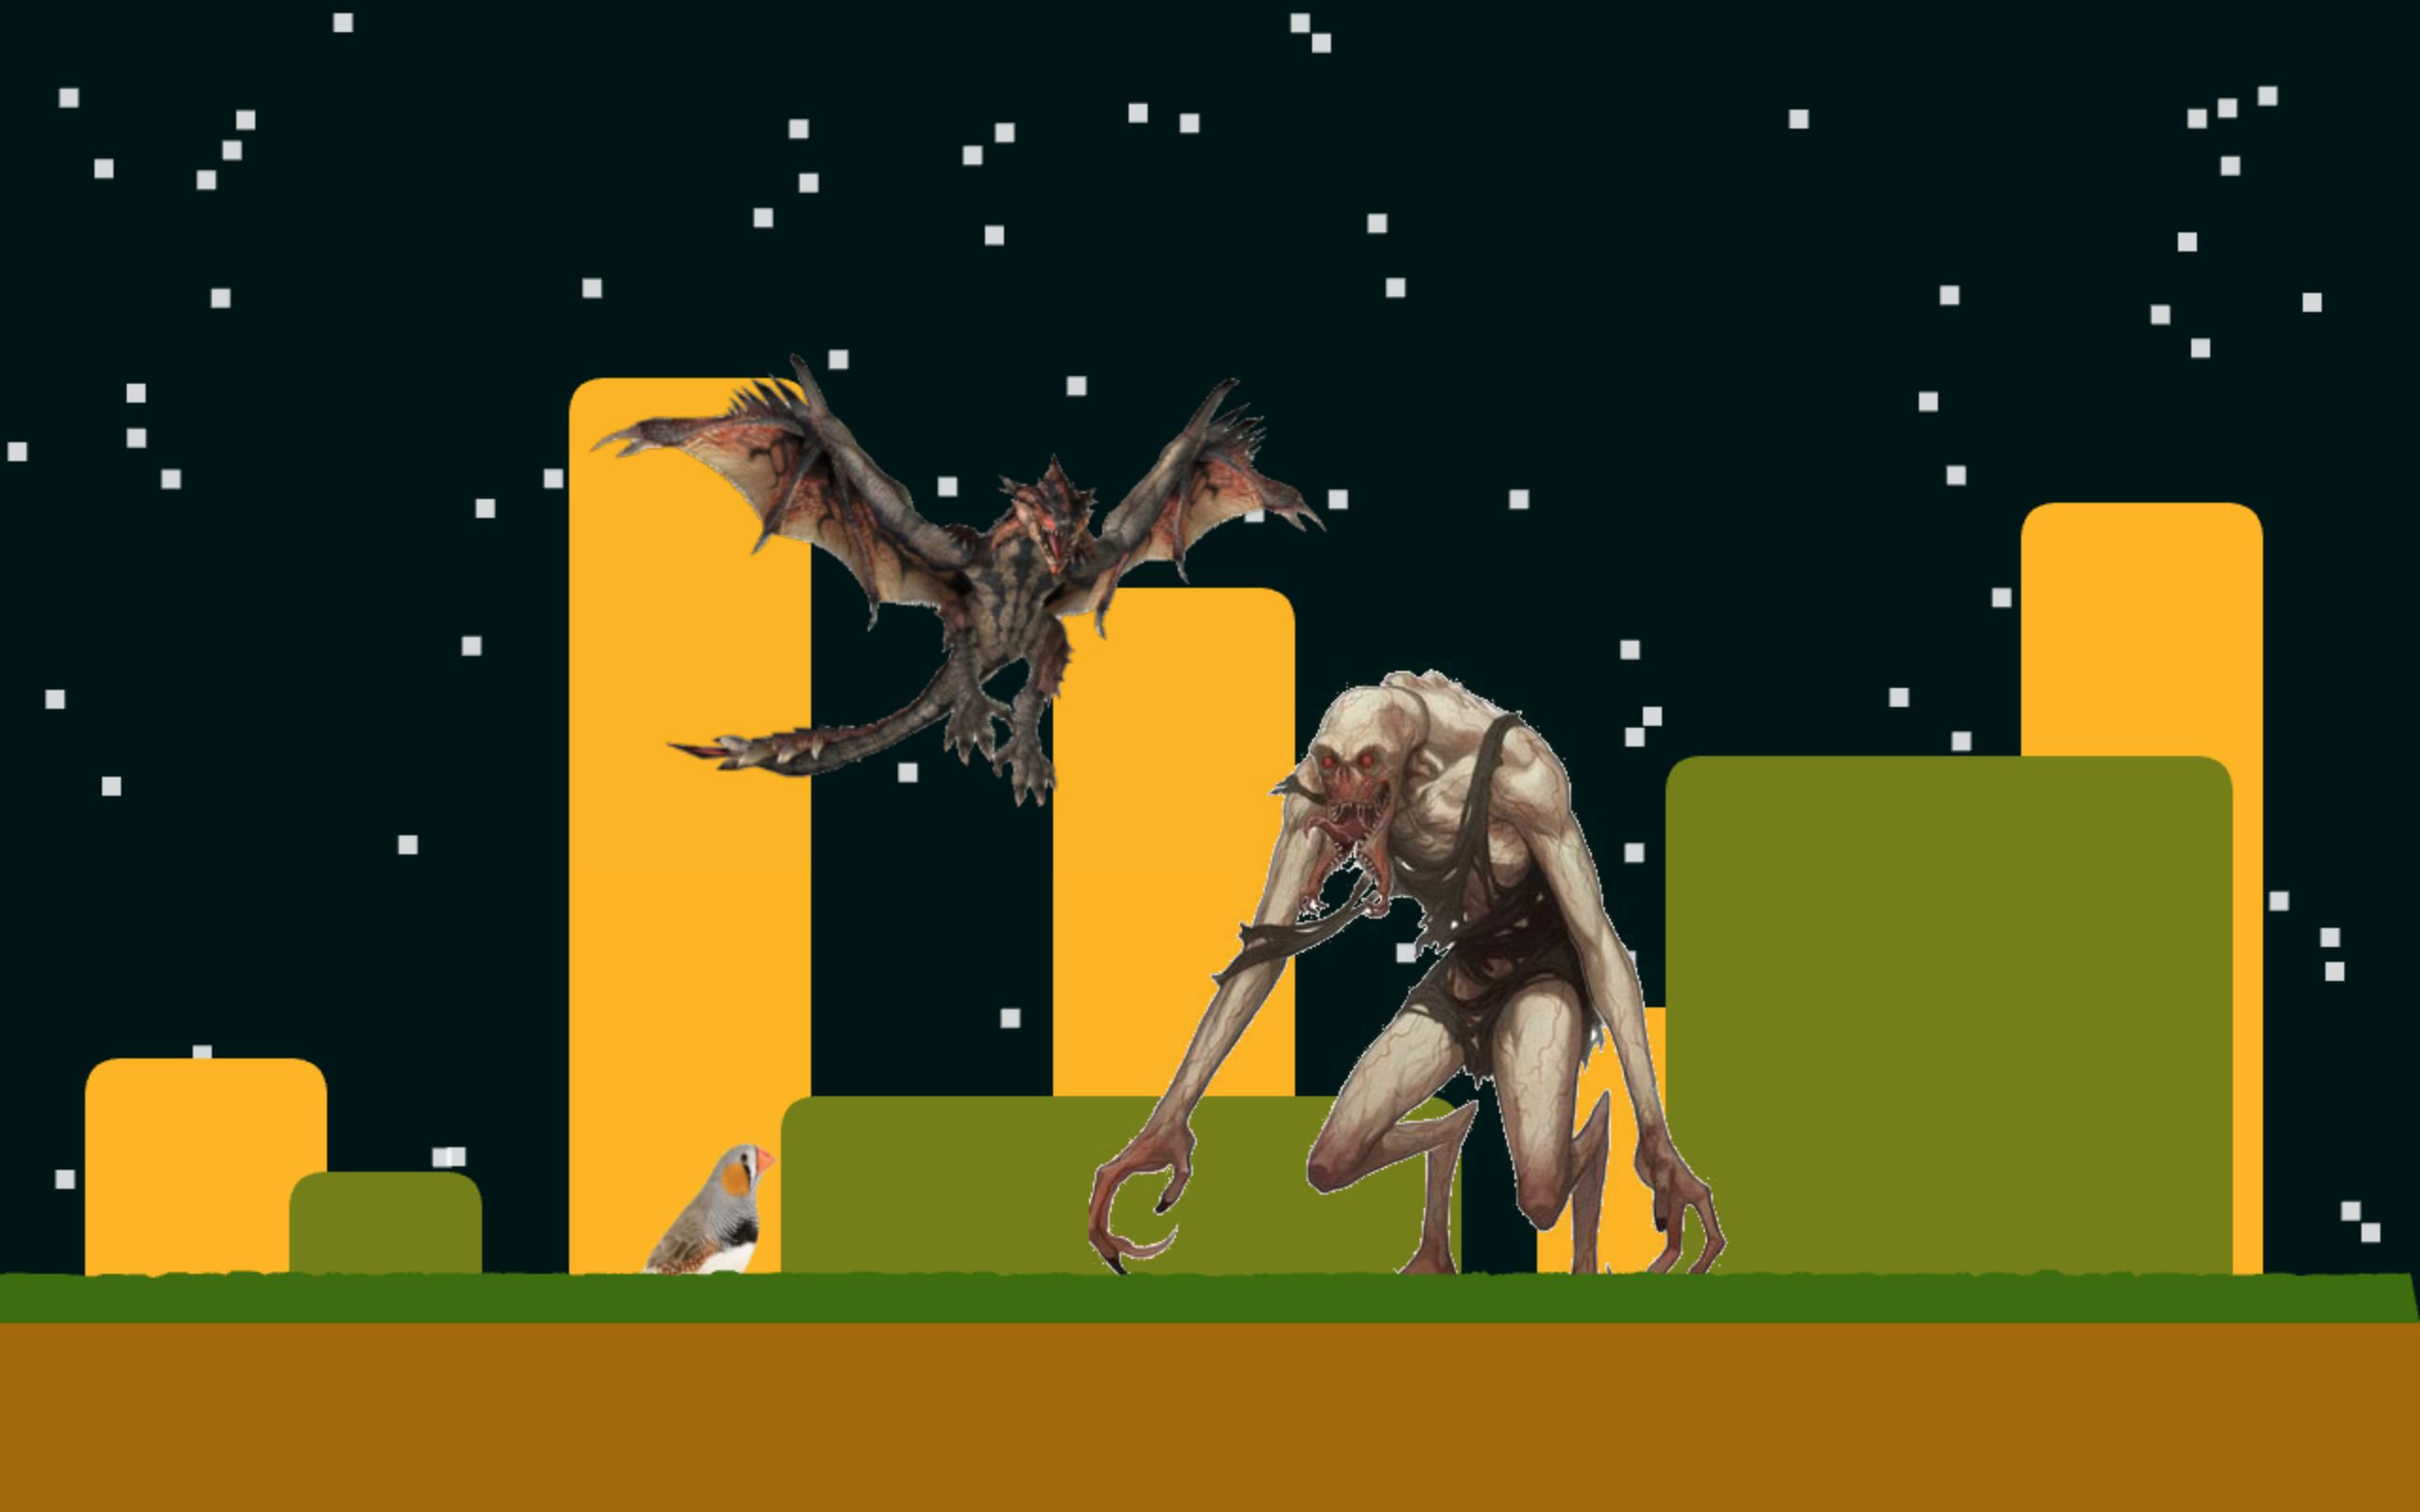
\includegraphics[scale=0.3]{pepper.png}
	\caption{\label{pepper} Screenshot from "Pepper".}
\end{figure}

\end{document}

